\section{Utilizzo}
	\subsection{Applicazione esterna a Grafana}
		\subsubsection{Aggiunta dei dati di addestramento}
		Per aggiungere i dati di addestramento si devono seguire i seguenti passo:
		\begin{enumerate}
			\item cliccare sul pulsante "Seleziona un file csv";
			\item si aprirà quindi il file manager di sistema da cui selezionare il file desiderato;
			\item ora apparirà un pop-up dove si deve:
			\begin{enumerate}
				\item scegliere l'algoritmo di predizione che si desidera l'addestramento dei dati;
				\item selezionare l'ordine dei predittori;
				\item selezionare l'ordine dei predetti.
			\end{enumerate}
		\end{enumerate}
		\mbox{}
		\begin{figure} [H]
			\begin{center}
				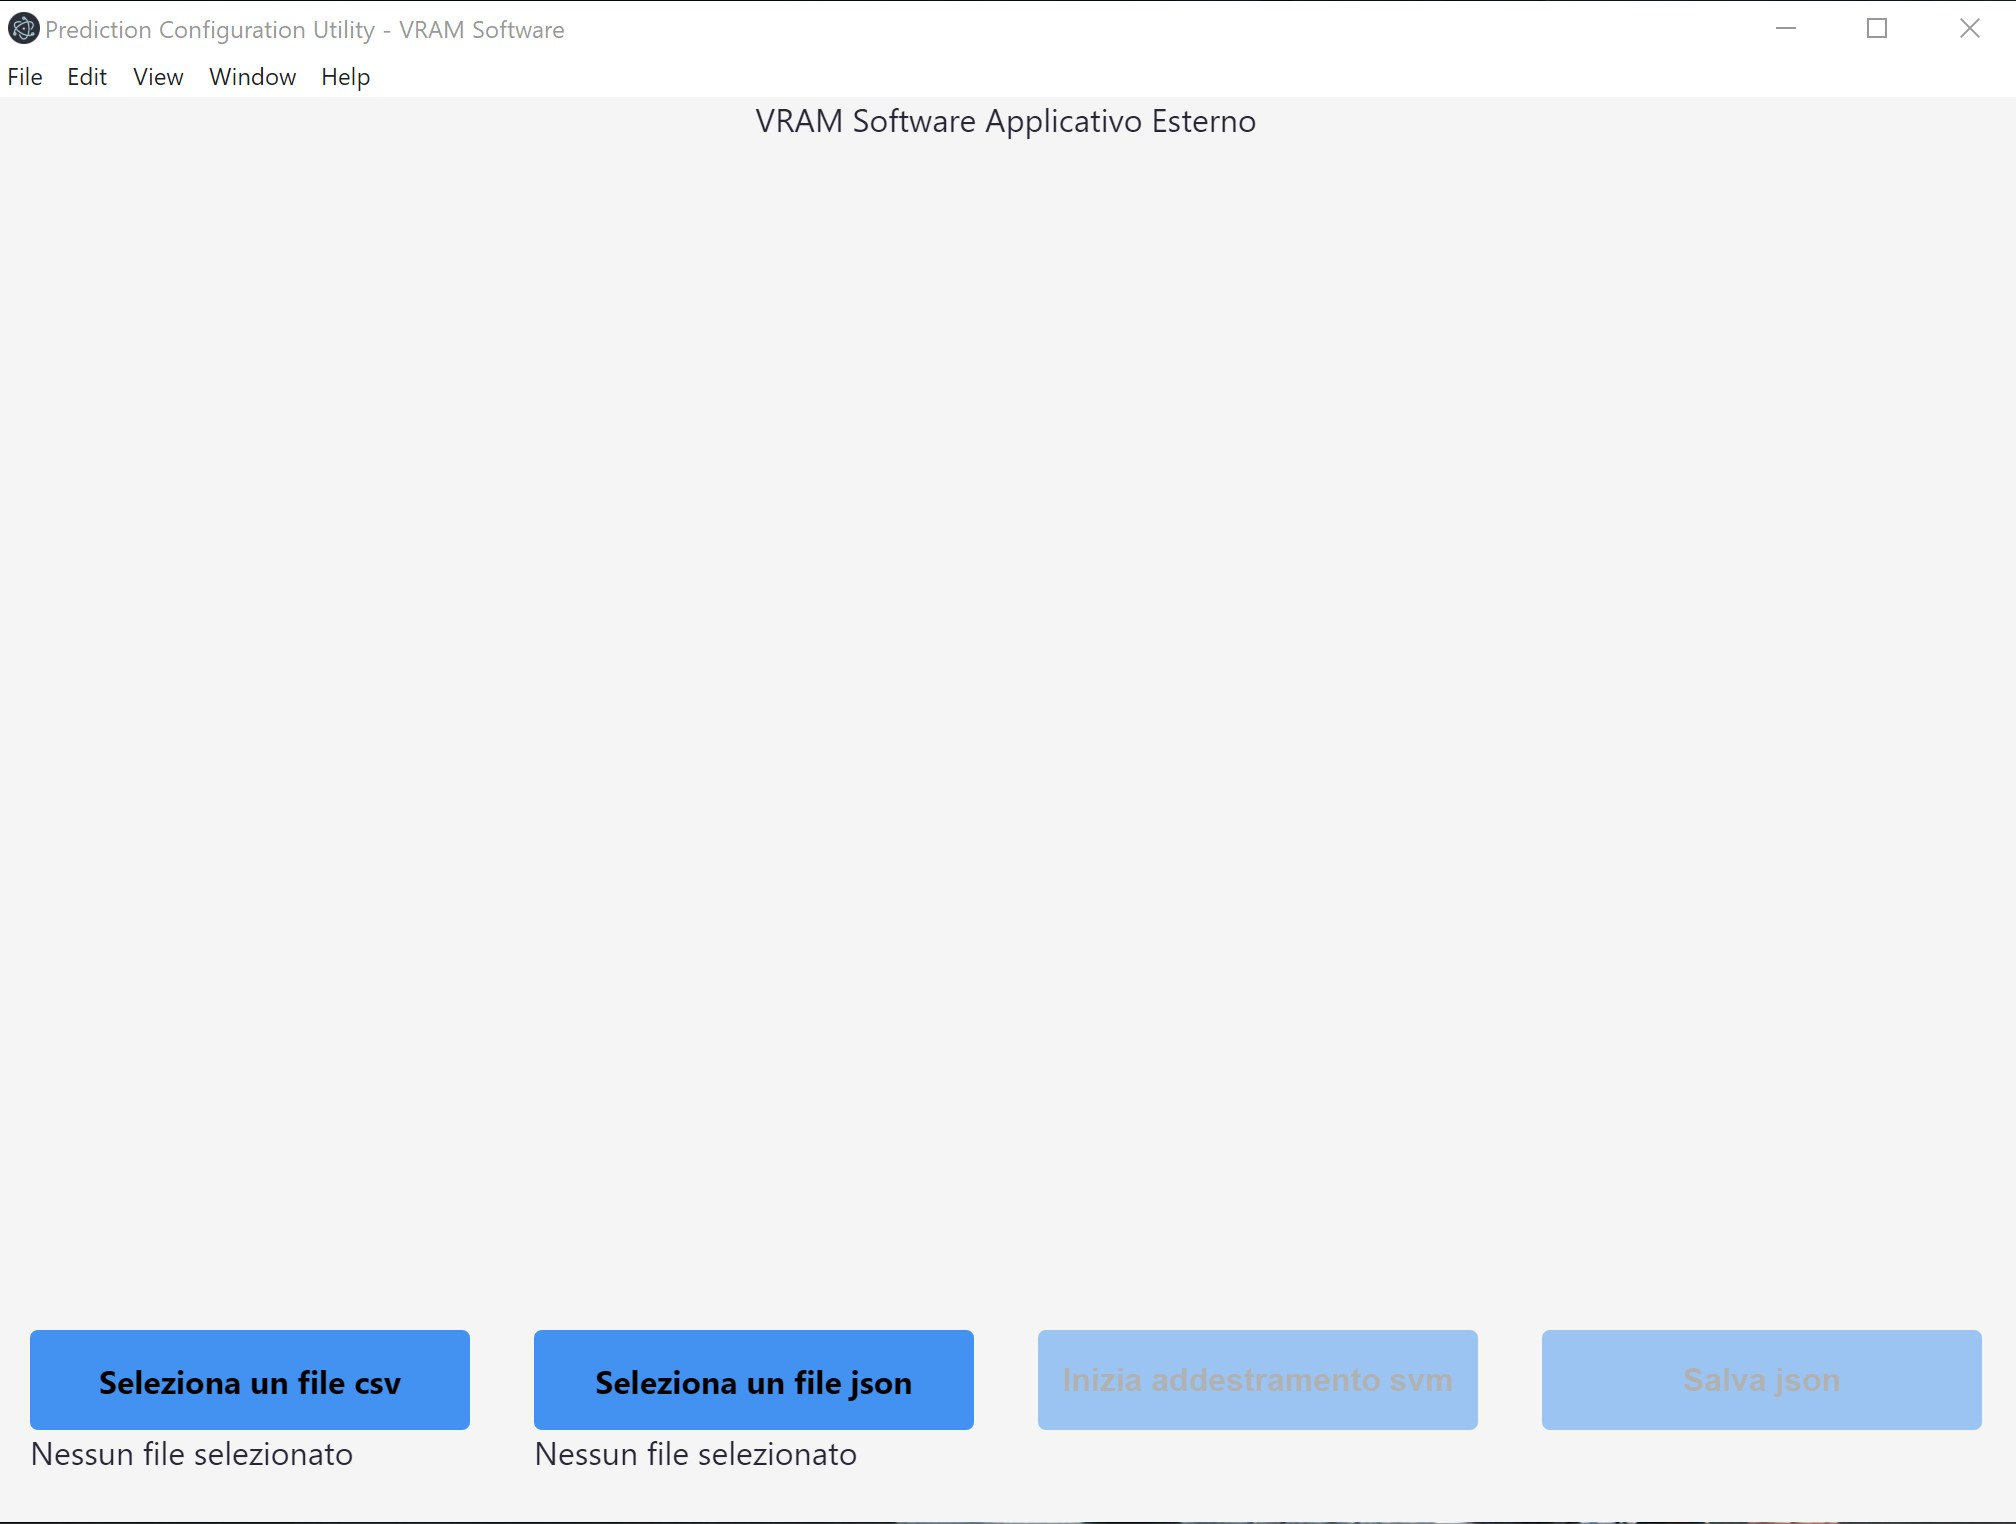
\includegraphics[width=120mm]{./img/1.jpg}
			\end{center}
			\caption{Pulsante Seleziona un file csv}
		\end{figure}
		\mbox{}
		\mbox{}
		\begin{figure} [H]
			\begin{center}
				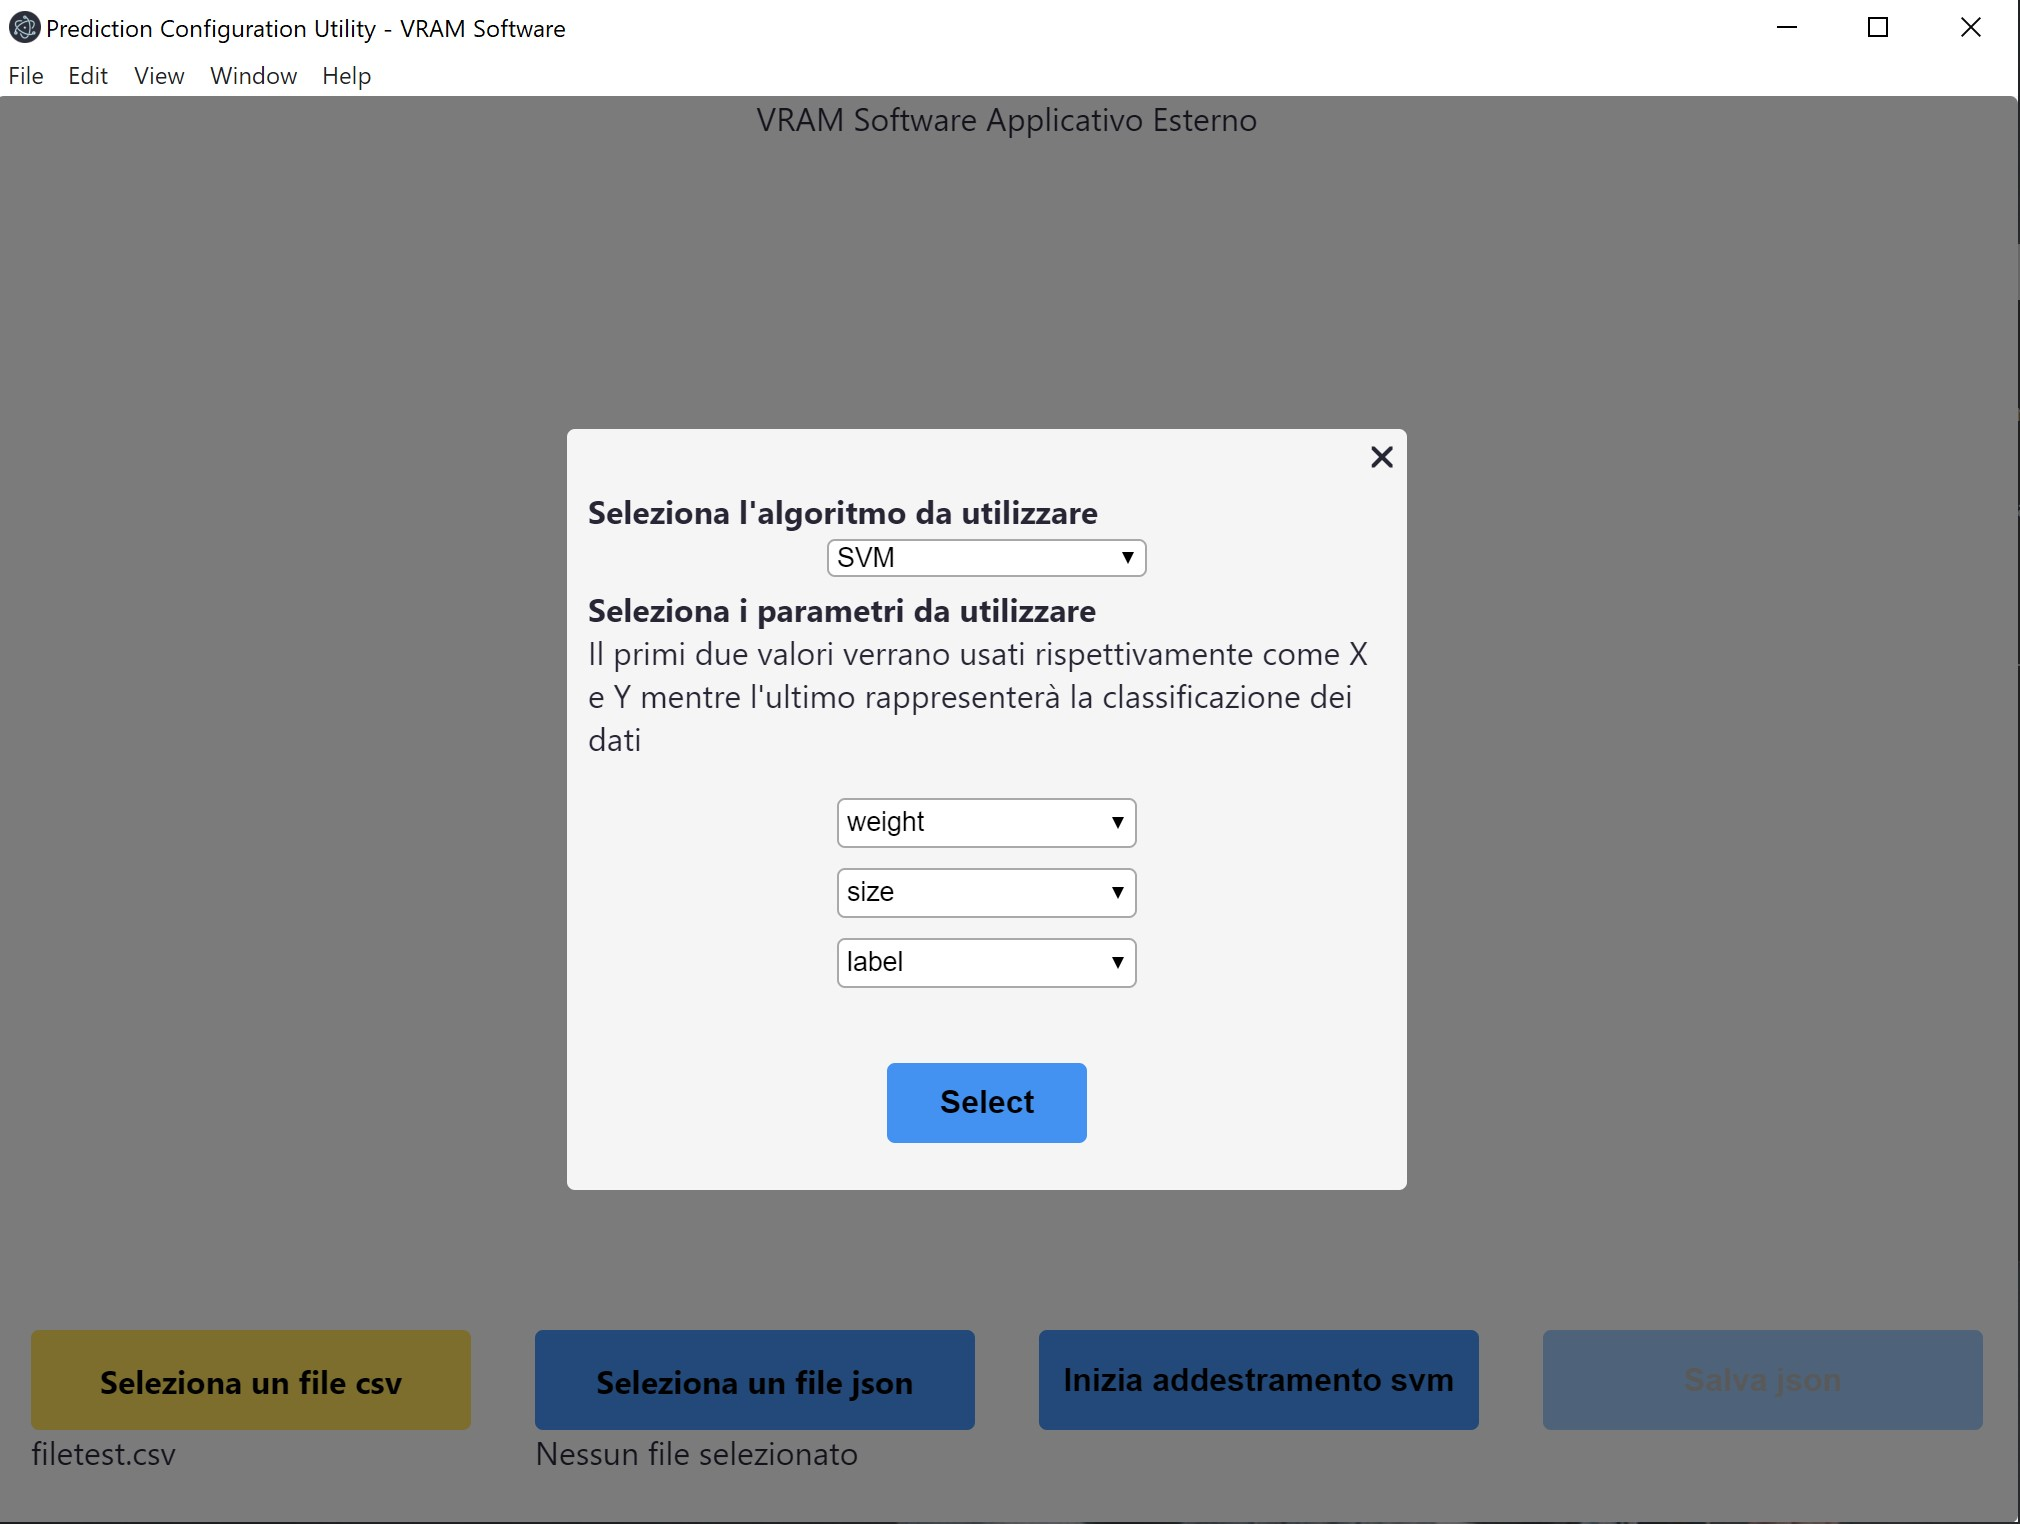
\includegraphics[width=120mm]{./img/2.jpg}
			\end{center}
			\caption{Scelta dei parametri}
		\end{figure}
		\mbox{}
		Una volta eseguita questa sequenza di operazioni, apparirà un grafico sulla base delle scelte effettuate.
		\subsubsection{Aggiunta di un file di configurazione}
		Per aggiungere un file di configurazione di un addestramento precedente è necessario eseguire le seguenti operazioni:
		\begin{enumerate}
			\item cliccare sul pulsante "Seleziona un file json";
			\item si aprirà quindi il file manager di sistema da cui selezionare il file desiderato;
			\item una volta selezionato, verranno automaticamente aggiornate le note dell'addestramento.
		\end{enumerate}
		\subsubsection{Avvio dell'addestramento}
		Solo dopo aver aggiunto i dati di addestramento è possibile avviarlo cliccando sul pulsante "Avvio addestramento". Al suo termine viene visualizzato il messaggio "Addestramento avvenuto" e, se le dimensioni dei dati lo consentono, il risultato sarà visualizzabile nel grafico.
		\mbox{}
		\begin{figure} [H]
			\begin{center}
				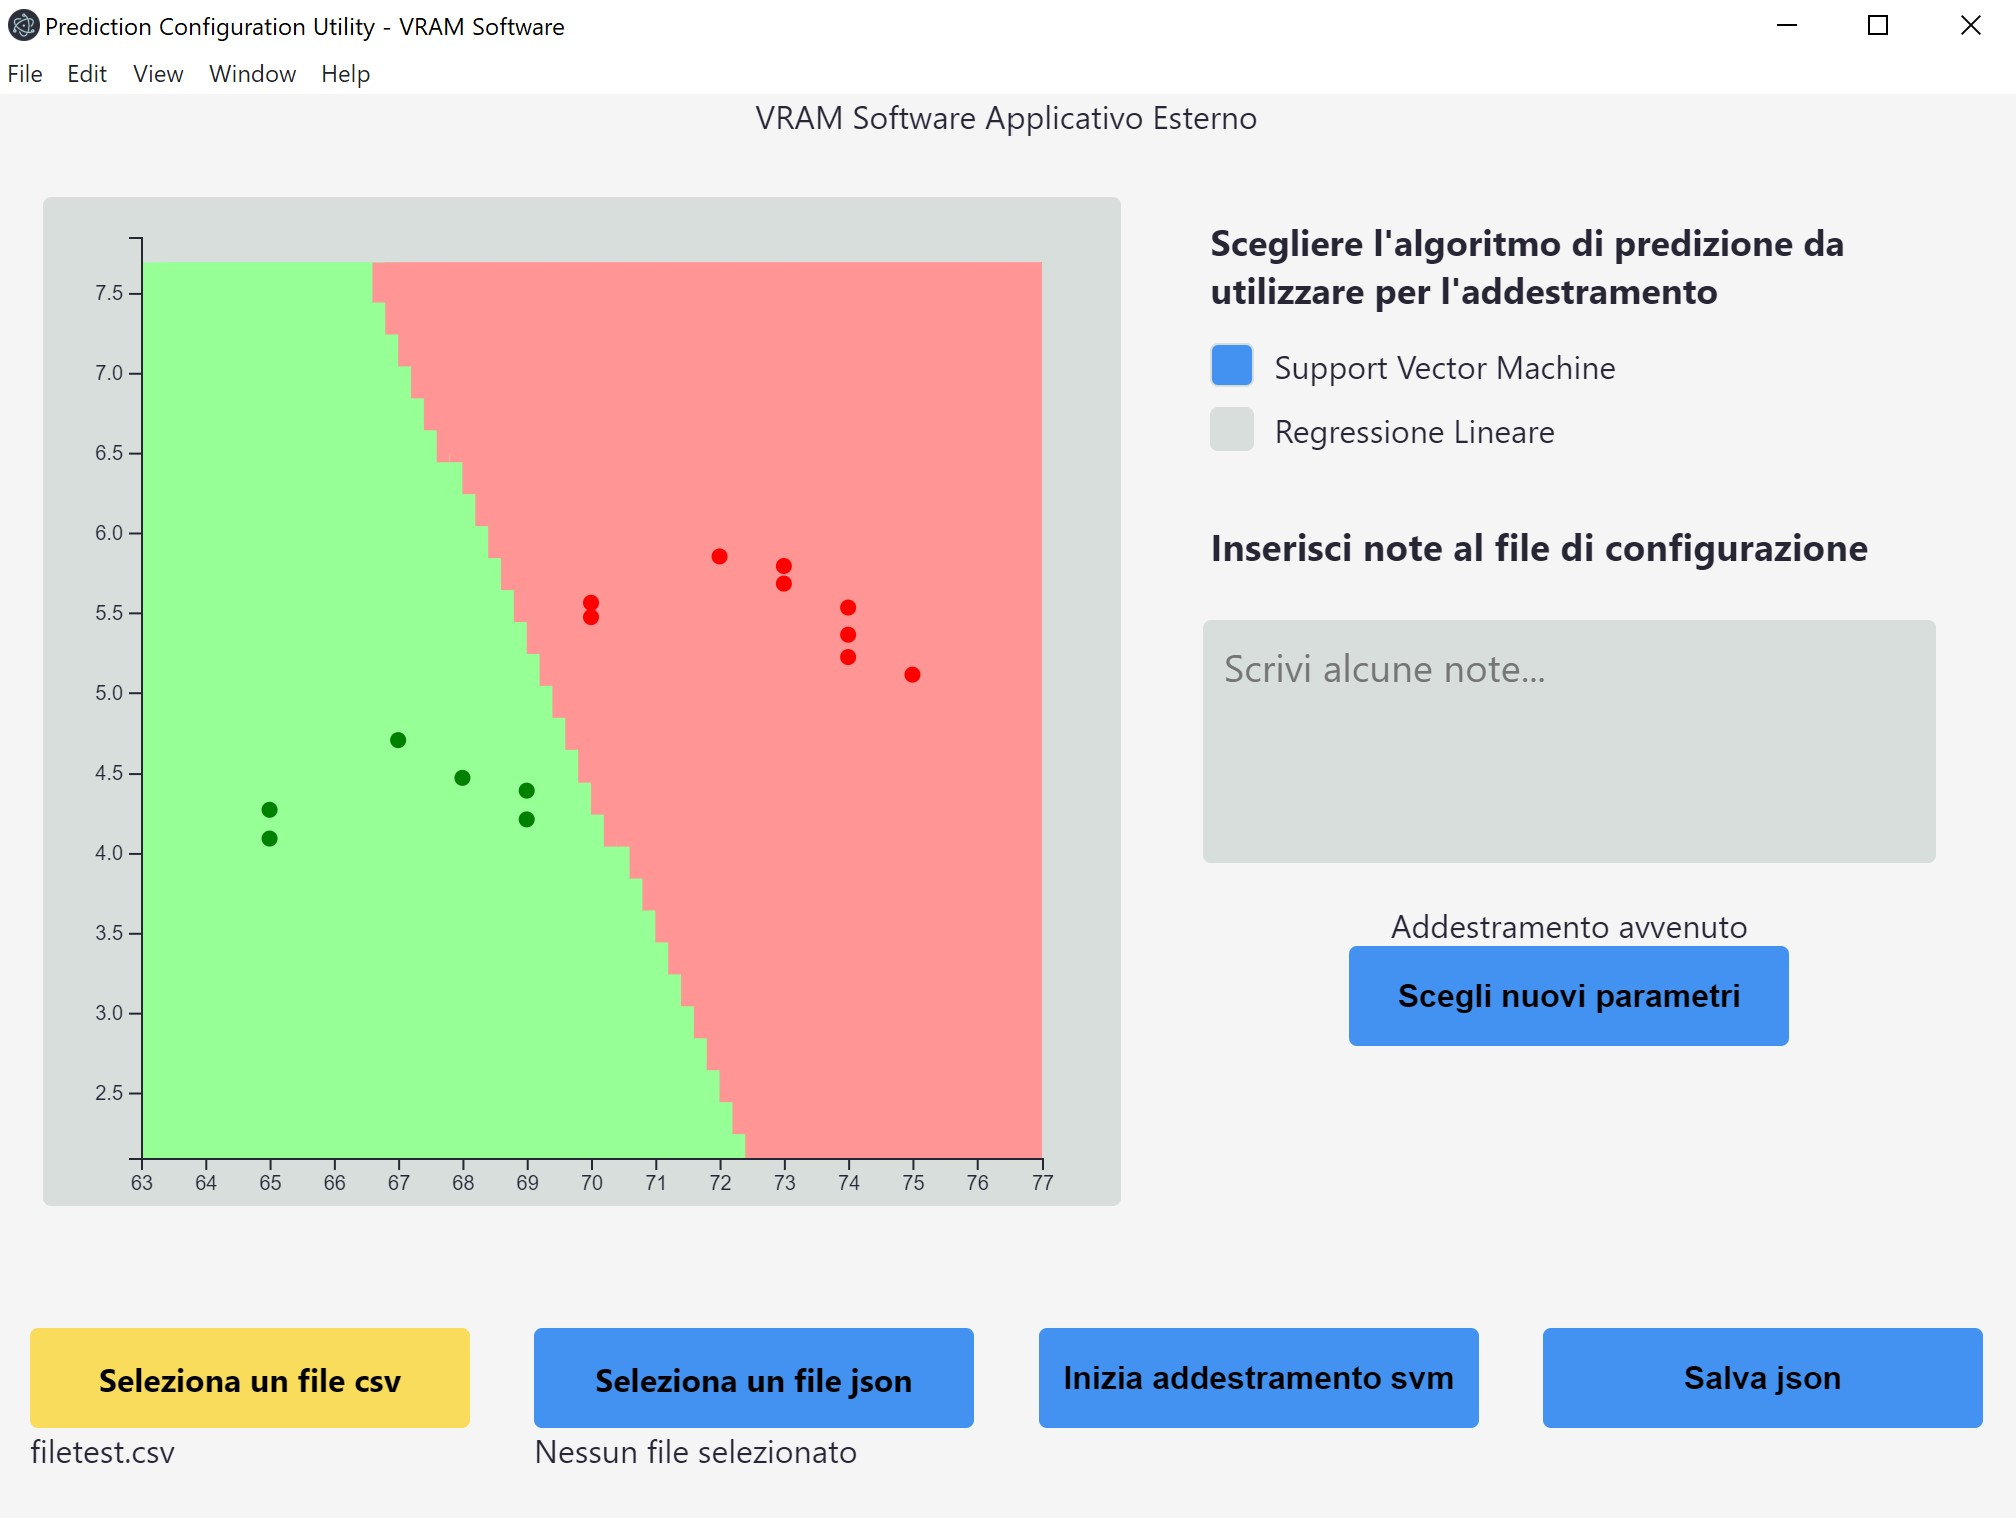
\includegraphics[width=120mm]{./img/4.jpg}
			\end{center}
			\caption{Addestramento avvenuto}
		\end{figure}
		\mbox{}
		\subsubsection{Cambio dei parametri}
		Nel caso si voglia cambiare i parametri dell'addestramento dopo aver già inserito il file csv si devo cliccare sul pulsante "Scegli nuovi parametri" e successivamente apparirà un pop-up. Qui sarà possibile cambiare l'ordine dei predittori e dei predetti come avviene nell'inserimento del file.
		\mbox{}
		\begin{figure} [H]
			\begin{center}
				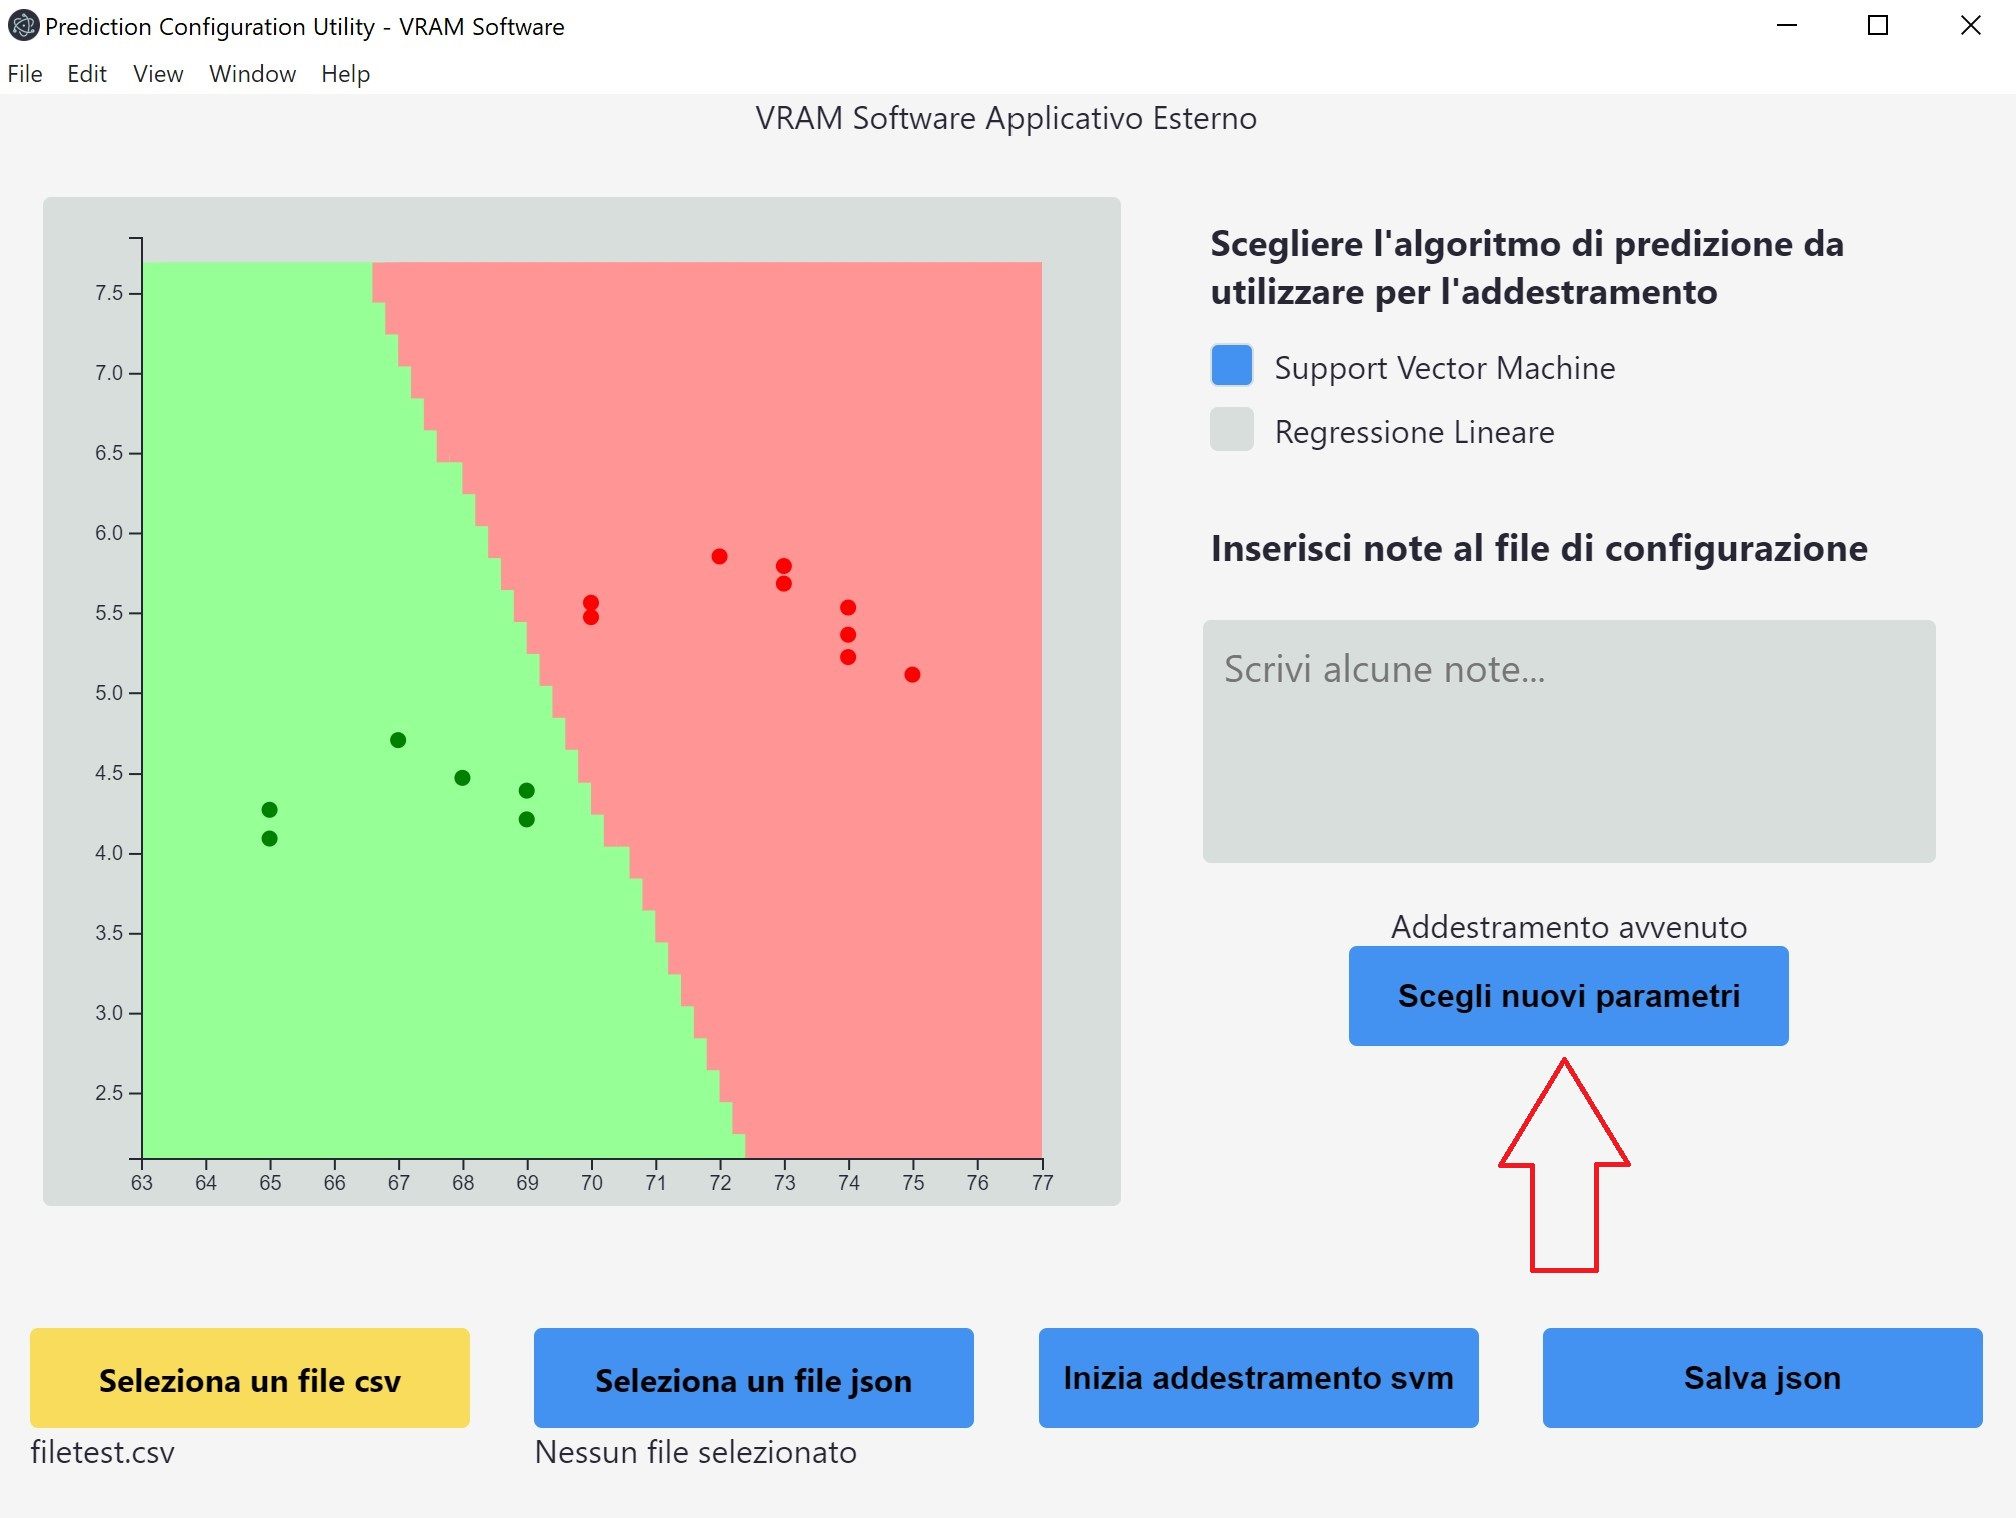
\includegraphics[width=112mm]{./img/4-1.jpg}
			\end{center}
			\caption{Pulsante Scegli nuovi parametri}
		\end{figure}
		\mbox{}
		\mbox{}
		\begin{figure} [H]
			\begin{center}
				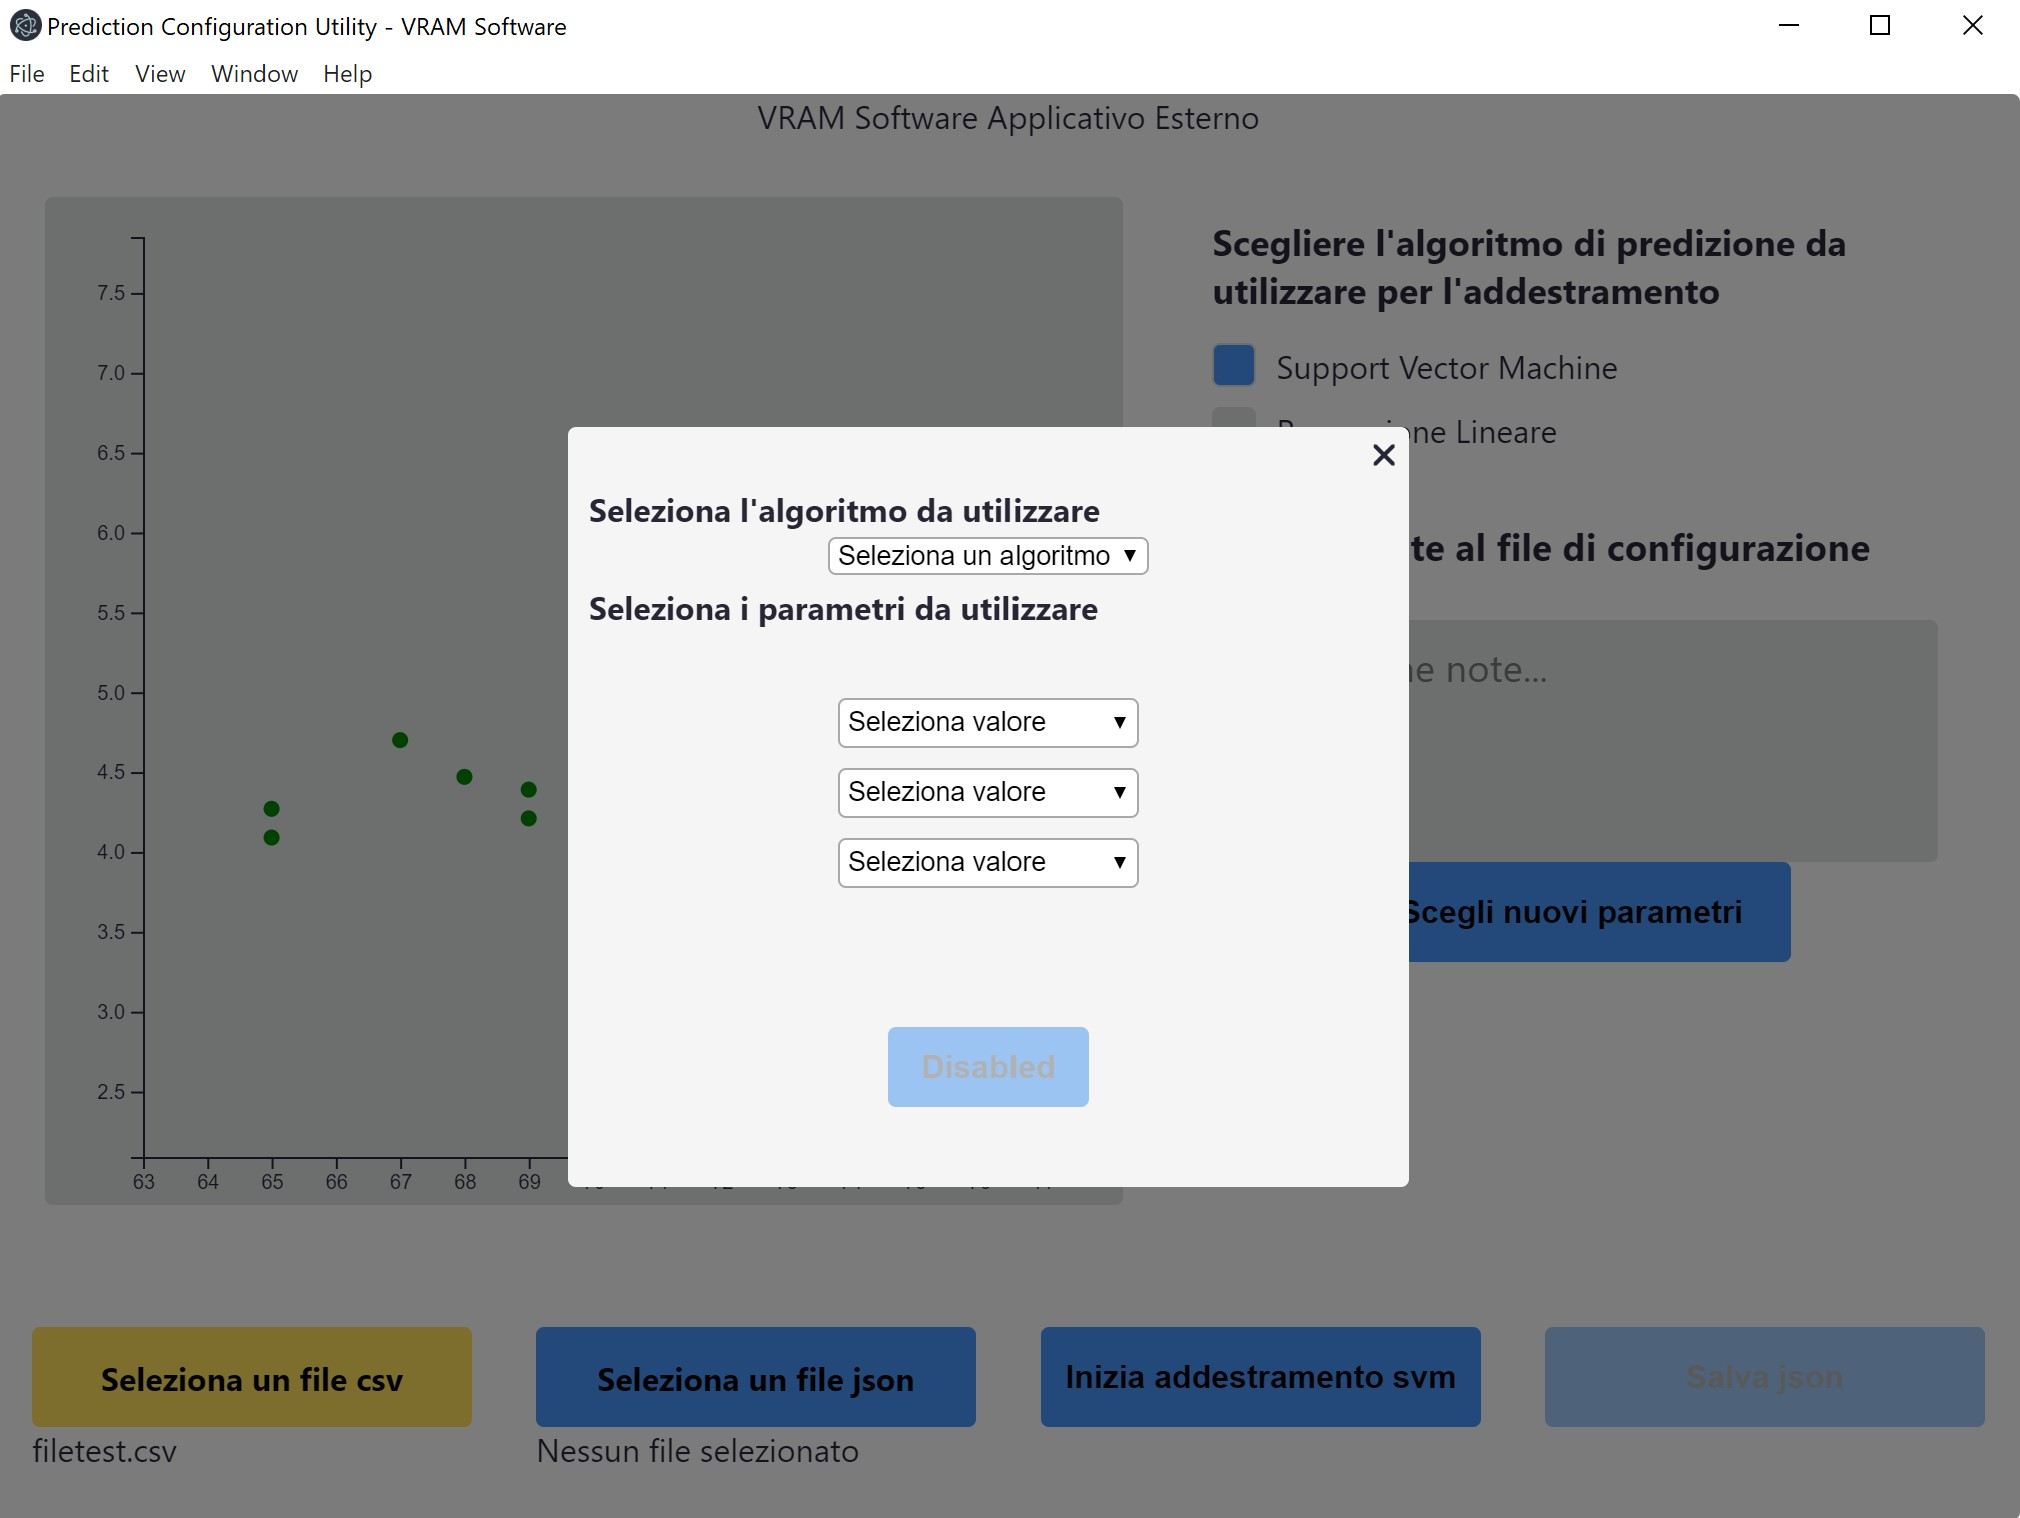
\includegraphics[width=112mm]{./img/3.jpg}
			\end{center}
			\caption{Cambio dei parametri}
		\end{figure}
		\mbox{}
		\subsubsection{Salvataggio dei risultati}
		Infine, solo dopo aver eseguito l'addestramento dei dati, è possibile salvare il risultato in un file Json. Si deve quindi cliccare sul pulsante "Salva json" e successivamente apparirà un pop-up in cui inserire il nome del file e salvarlo sulla cartella "output". Questo file conterrà tutte le informazioni dell'addestramento necessarie per eseguire la predizione oltre alle eventuali note scritte nel box dell'applicazione.
		\mbox{}
		\begin{figure} [H]
			\begin{center}
				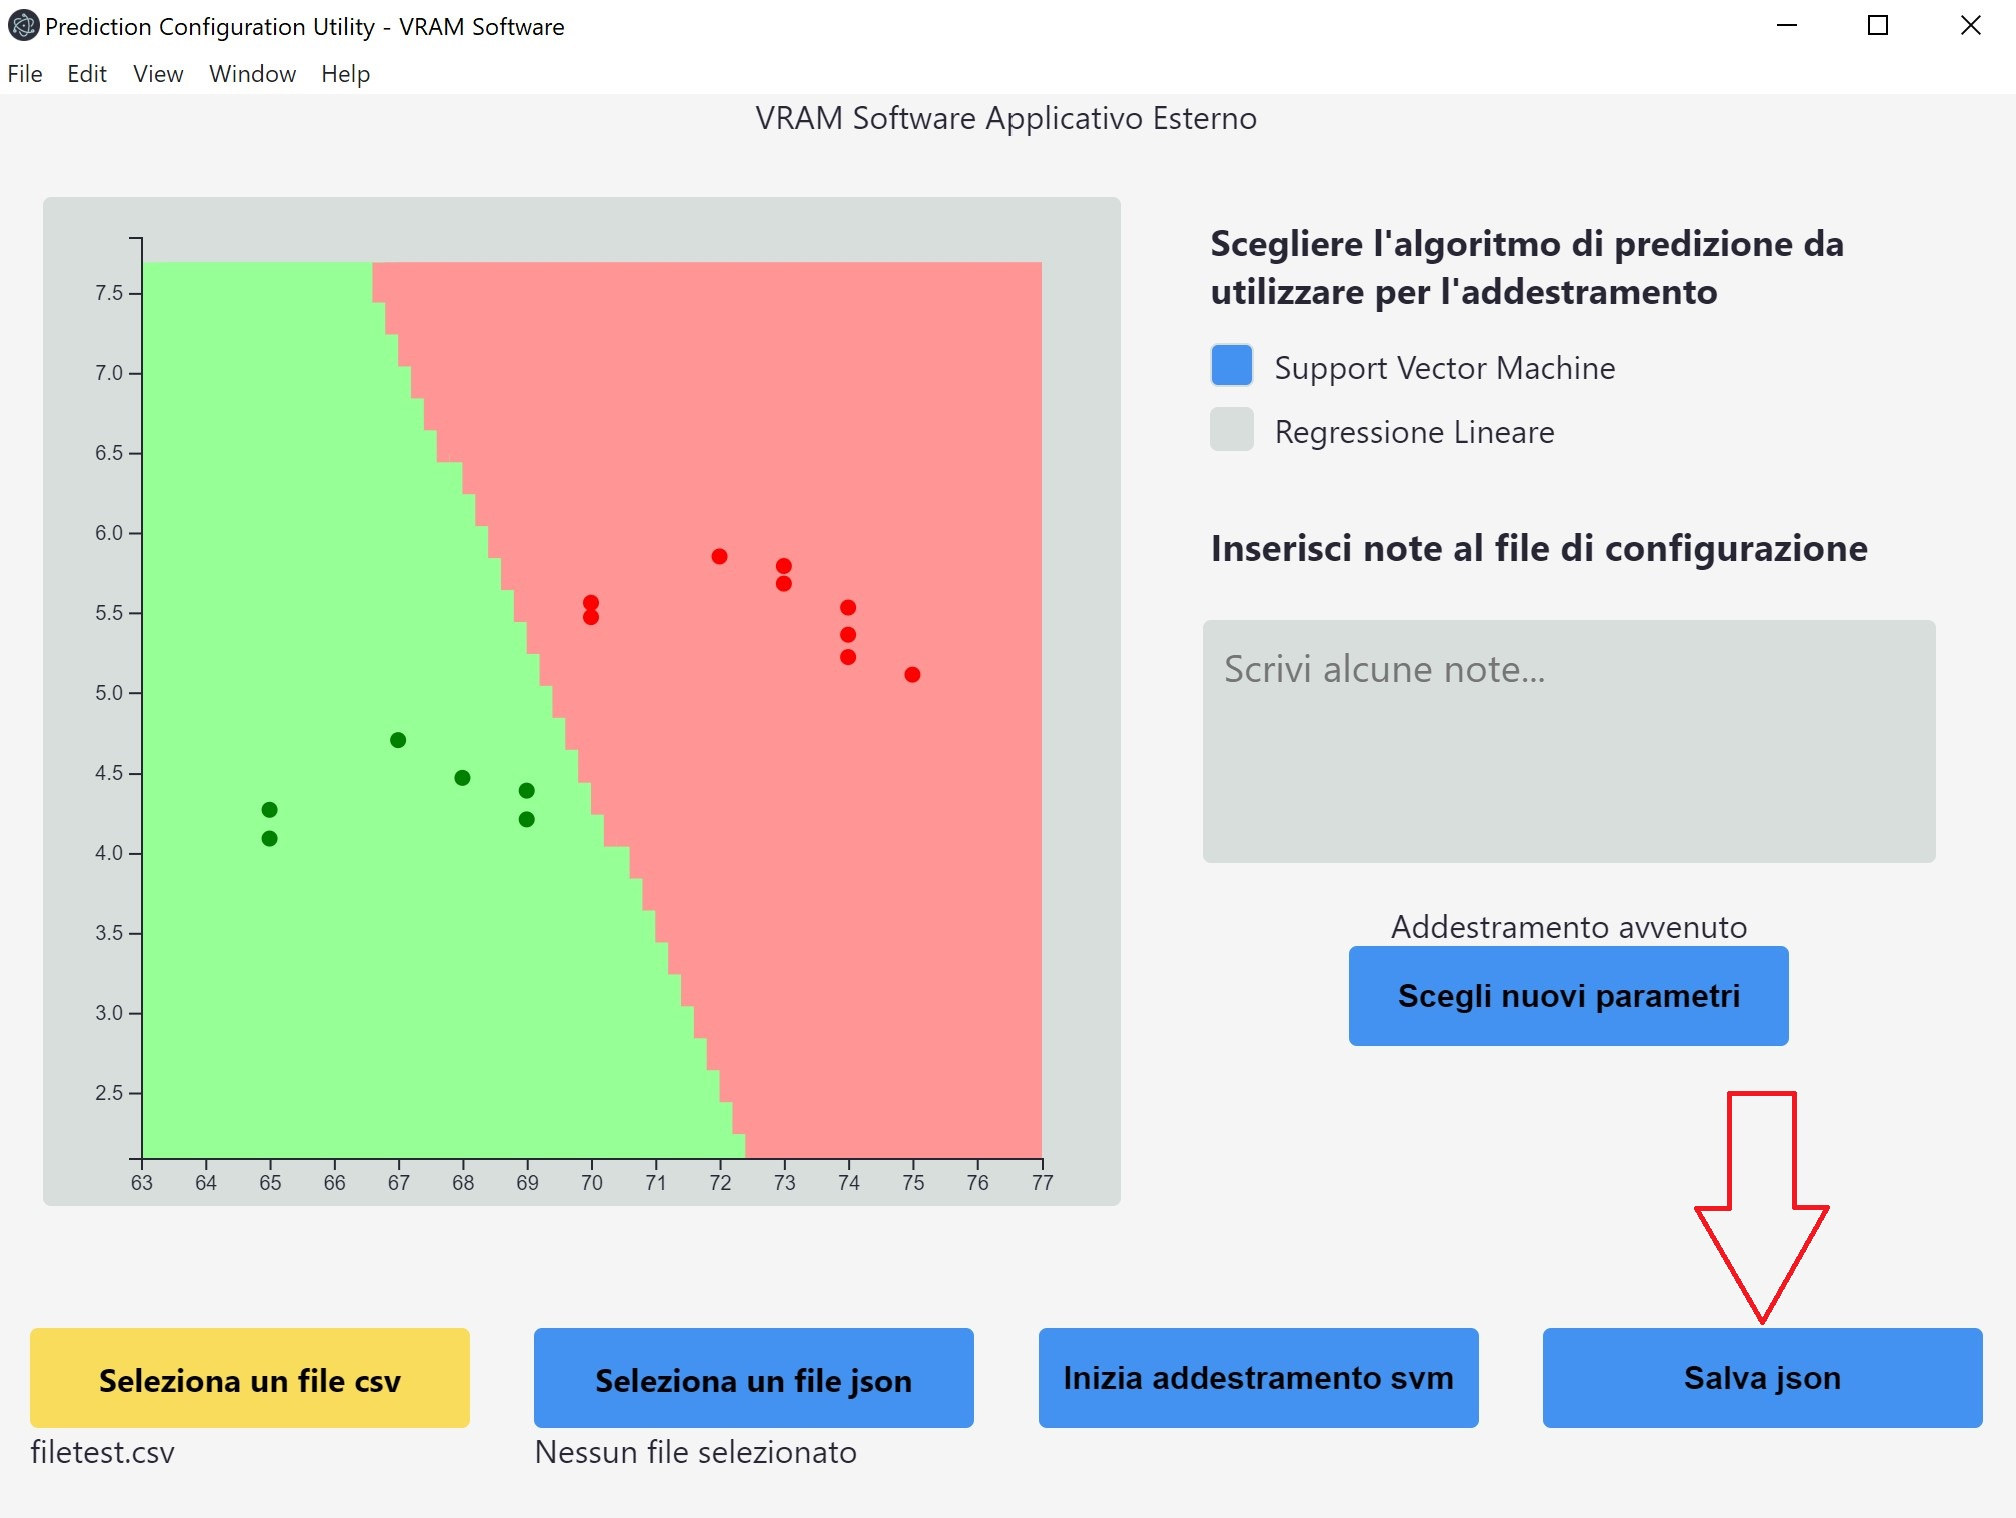
\includegraphics[width=112mm]{./img/4-2.jpg}
			\end{center}
			\caption{Pulsante Salva json}
		\end{figure}
		\mbox{}
		\mbox{}
		\begin{figure} [H]
			\begin{center}
				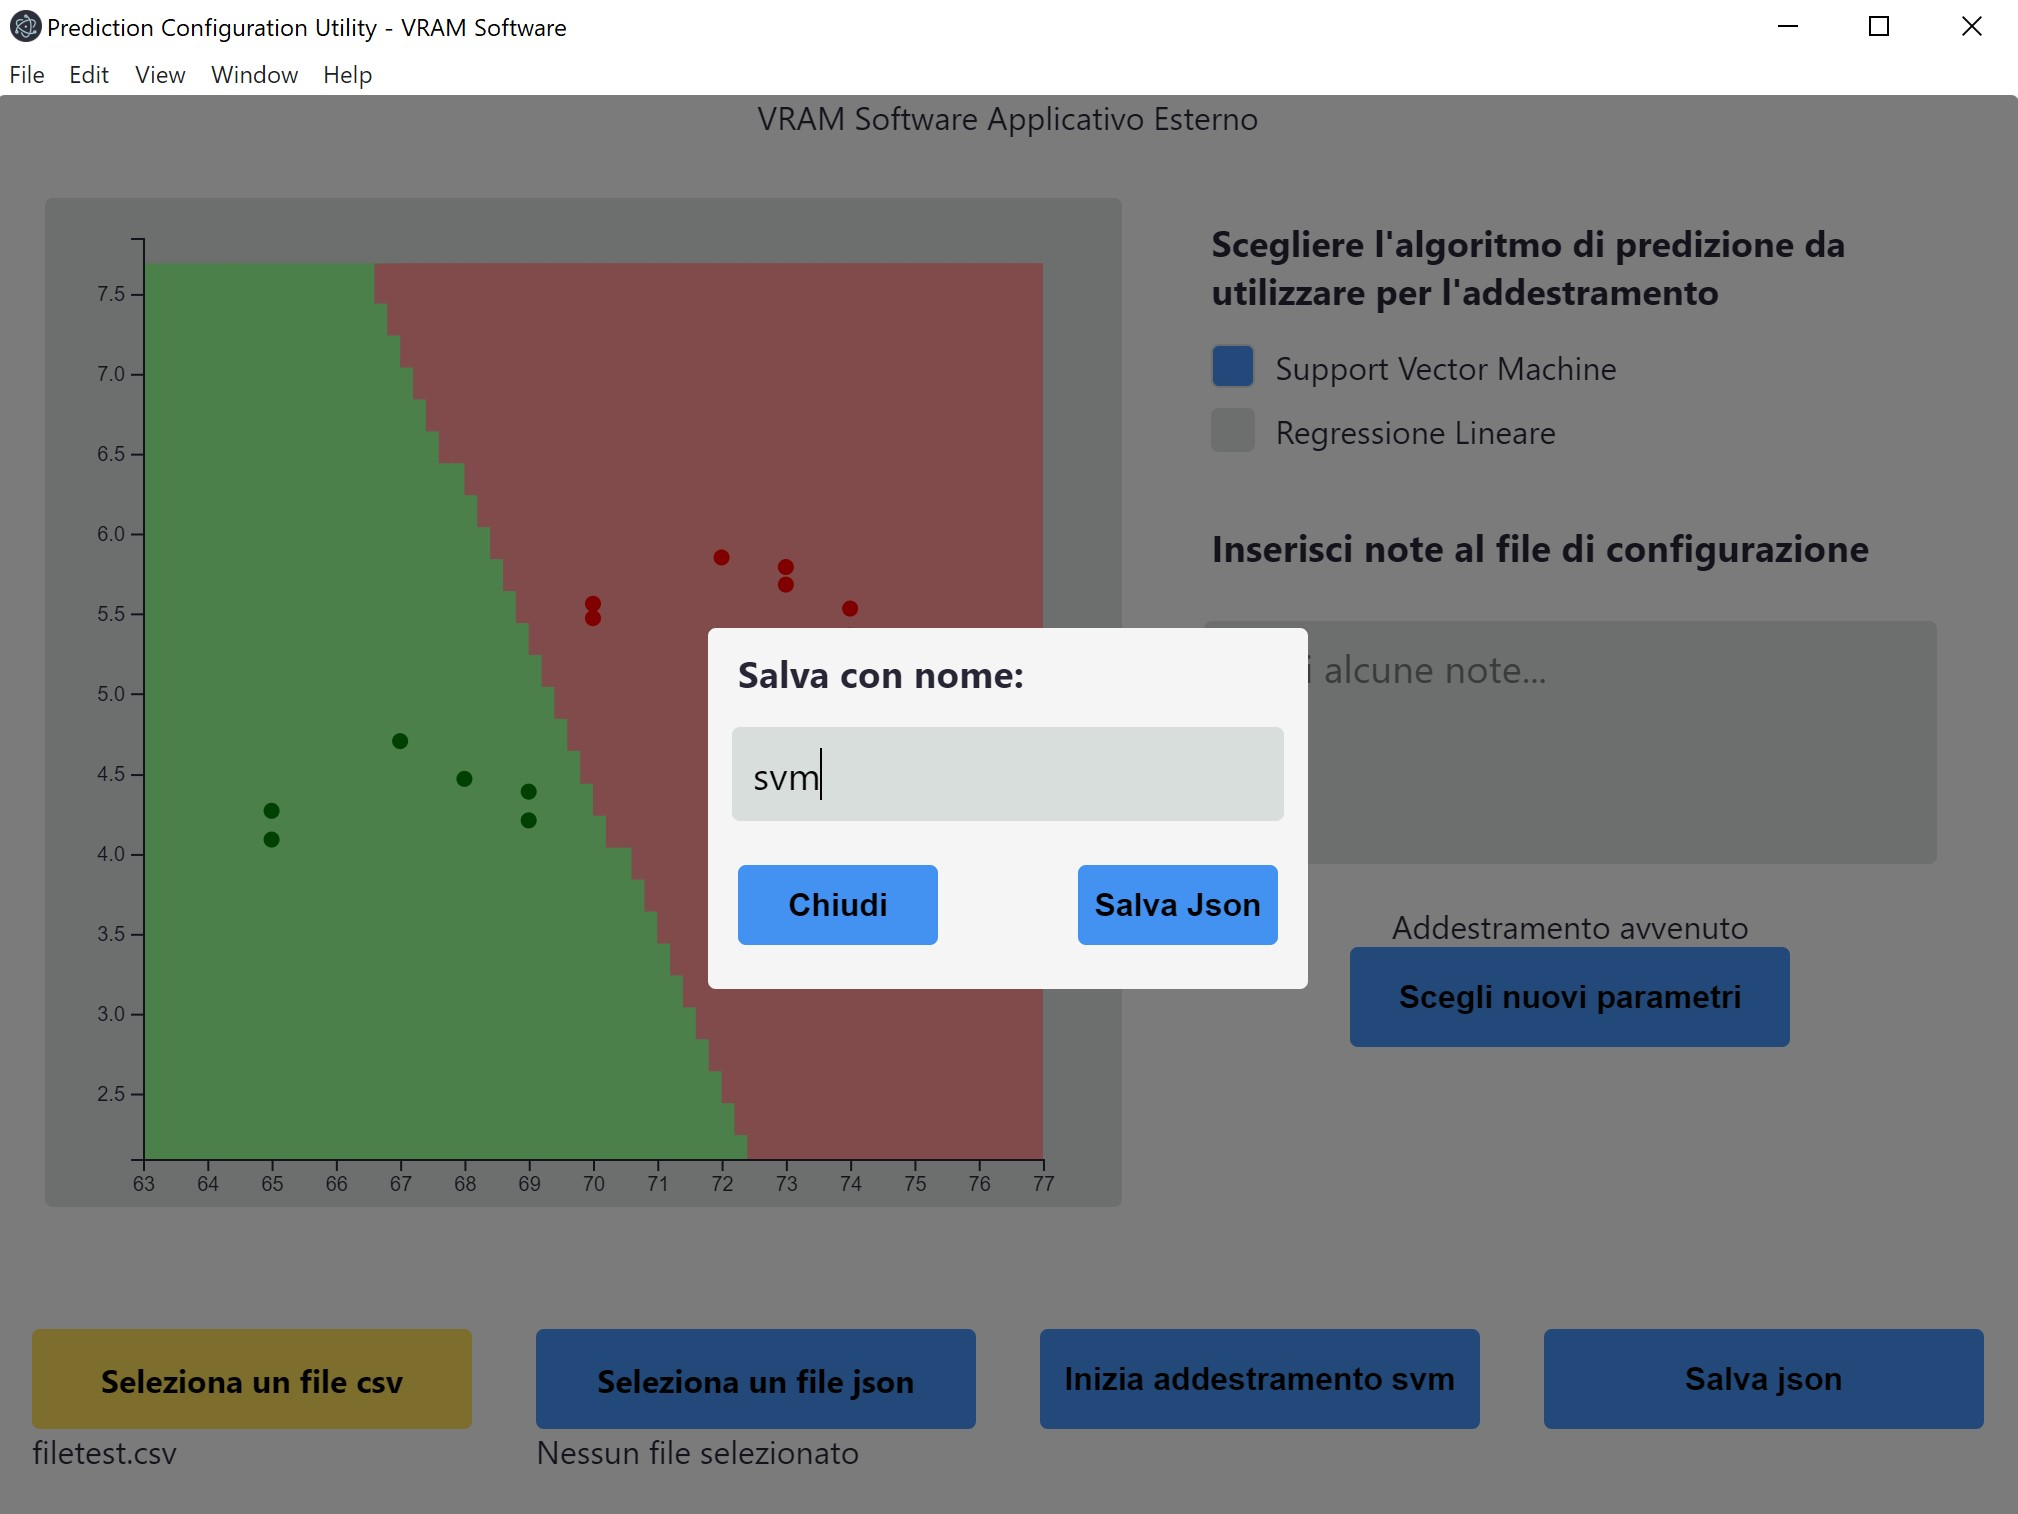
\includegraphics[width=112mm]{./img/5.jpg}
			\end{center}
			\caption{Salvataggio del file json contenente la configurazione per la predizione}
		\end{figure}
		\mbox{}
		
